\documentclass[12pt]{article}
\usepackage[utf8]{inputenc}
\usepackage[T1]{fontenc}
\usepackage[left=2cm,right=2cm,top=2cm,bottom=2cm]{geometry}
\usepackage[french]{babel}
\usepackage{graphicx}
\usepackage{url}
\usepackage{hyperref}
\hypersetup{
    colorlinks,
    citecolor=black,
    filecolor=black,
    linkcolor=black,
    urlcolor=black
}
\bibliographystyle{alpha}


\begin{document}
	\begin{titlepage}
		
\includegraphics[scale=0.2]{logo_bordeaux.png}\\
		\centering
		{\LARGE \bfseries Université de Bordeaux}\\ [2cm]
		\textsc{\Large Master 1 Informatique}\\ [0,3cm]
		\textsc{\Large 2016/2017}\\ [1,5cm]

		\textsc{\Large Projet de programmation}\\ [1.5cm]


		\rule{16cm}{1mm}\\ [0,7cm]
		{ \huge \bfseries Visualisation de trajets de vélos en libre service} \\[0,5cm]
		{ \huge \bfseries Analyse des besoins}\\ [0,7cm]
		\rule{16cm}{1mm}\\ [1cm]

		{\Large Chargé de TD Boris MANSENCAL }\\ [0,3cm]
		{\Large Client Romain GIOT }\\ [1cm]

		{\Large Damien Bielawski }\\ [0,3cm]
		{\Large Sébastien Bielawski }\\[0,3cm]
		{\Large Alaric Braillon }\\ [0,3cm]
		{\Large Alassane Diop }\\ [2cm]
		\Large\today

	\end{titlepage}

	\tableofcontents \newpage

	\section{Introduction}
		Cette section a pour but de décrire et donner un aperçu sur le contenu de ce document d'analyse des besoins. Il présente aussi les cherches et ce qui a déjà été fait sur ce sujet.

		\subsection{Contexte}
			Le projet consiste en la réalisation d’un logiciel de visualisation de trajets d'un système de vélos en libre service. 
			Il est réalisé par quatre étudiants de première année de master informatique, dans le cadre d'une UE de projet de programmation.

		\subsection{Objectifs}
			Ce logiciel doit permettre la visualisation des fonctionnement des systèmes de vélos en libre service. En utilisant les données mise à disposition par les villes et par des données récuperables sur les web, on peut récuperer les informations sur les trajets des utilisateurs dans une ville donnée.\\
			Le logiciel est destiné aux personnes souhaitant analyser les trajets d'un système de vélos en libre service, grâce à des données libres. Il peut permettre l'analyse statistique des trajets, comme connaître le temps moyen d'un trajet des utilisateurs par exemple.

		\subsection{Définitions, acronymes}
			BSS : bike sharing system\par
			CSV : Comma Separated Value, c'est un format de fichier\par
			JSON : format de fichier

		\subsection{Description de l'existant}
			Une application a déjà était développé par des chercheurs. Il s’agit d’une application web qui a l’inconvénient d’être assez lente dès lors qu’il y a beaucoup de donnée à traiter. Les liens vers les deux vidéos montre qu'il s'agit d'une application web ouverte avec Google Chrome. On peut aussi voir d'après l'url, qu'il s'agit d'une démonstration en local (localhost:8080). Nous supposons que les performances ne doivent pas être optimales avec ce type de technologie pour le web. Cependant nous ne savons pas combien de données ont été utilisées pour la demonstration.\\*\\*
			Aperçu de ce qui existe.\\*
			\url{https://drive.google.com/file/d/0B3aeg8yMfRj0MWFmUHZ6ZlR4MzA/view}\\*
			\url{https://drive.google.com/file/d/0B3aeg8yMfRj0R3VKQjdtX1htUUU/view}
		
		\subsection{Réferences}
			\begin{itemize}
				\item L'article \cite{Oli16} donne un aperçu sur les différentes interfaces à implémenter dans notre logiciel. Ce sera le document sur lequel nous nous reposerons le plus.

				\item L'article \cite{Ali14} explique comment détecter les stations les plus connectées. Donne un aperçu sur comment utiliser des filtres (date, lieu, heure...).

				\item \cite{BC16} est un article sur les systèmes de partage de vélos. Il parle de l'application FunFEM qui permet de visualiser des données afin de juger de l'efficacité de ces systèmes.

				\item \cite{BSM17} est une application en ligne, qui permet de visualiser le nombre de bornes disponible dans une ville ainsi que le nombre de vélos disponible sur celle-ci.

				\item L'article \cite{BW} de Ben Wellington, nous donne un bel aperçu sur comment l'analyse statistique des données sur les utilisateurs du système de vélos en libre service peut être utilisé. Il montre comment les societés qui mettent à disposition les vélos dans la ville de New York, pourraient augmenter leurs revenus grâce à une analyse des trajets des utilisateurs.

			\end{itemize}
			
	\section{Expression des besoins}
		Cette section fournie une déscription detailée des fonctionnalités du logiciel.
		\subsection{Besoins fonctionnels}
			Visualiser la carte d’une ville choisie par l'utilisateur.\\*
			Charger des trajets depuis un fichier (les formats acceptés seront définis ultérieurement).\\*
			Supprimer un trajet de la fenêtre de visualisation.\\*
			Visualiser les trajets chargés, \\*
			Filtrer les trajets selon certains critères (critères spatio-temporels, type de trajet (départ, arrivée, cycle), fréquence d'utilisation des vélos).

		\subsection{Besoins non fonctionnels}
			Le code doit être bien conçu avec un bon nommage des variables et des fonctions afin qu'il soit facile à comprendre pour un développeur qui n'a pas travaillé sur le projet.\\*
			Il doit aussi être bien documenté, l'architecture doit permettre d'étendre facilement de nouveaux systèmes de visualisation ainsi que de nouvelles fonctionnalités.\\*
			Il faut que l'application dispose d'une bonne base afin que le code soit repris et amélioré par une autre équipe.

	\section{Contraintes}
		\begin{itemize}
			\item Langage : C++14 pour concilier la performance (afin de gérer des centaines de miliers de trjets) et la lisibilité.
			\item Framework Qt pour l'interface graphique : c'est aussi un éditeur de d'interaface graphique qui permet de créer l'interface graphique à la manière WYSIWIG.
			\item L'API OpenGL pour le rendu des nombreux trajets.
			\item C++14, Qt et OpenGL permettent également la portabilité sous Linux, MacOS et Windows.
		\end{itemize}

	\section{Les livrables}
		Une fois le delai passé, le code source bien commenté ainsi qu'un fichier exécutable sera remis. En plus de cela une documentation détaillée sur la manière d'utilisée le logiciel sera mis à disposition.

	\section{Prototypes}
		\begin{figure}[!ht]
		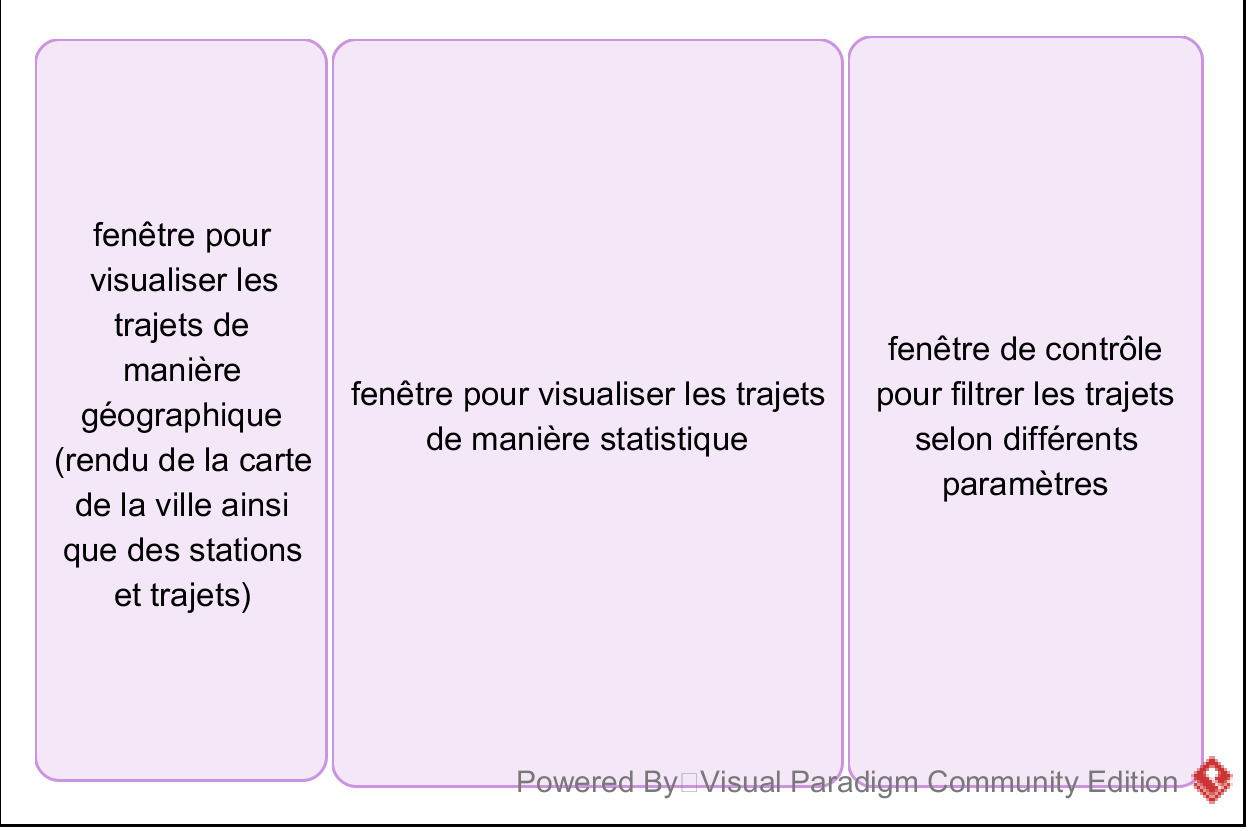
\includegraphics[scale=1.2]{proto_interface1.png}
		\caption{Prototype d'interface graphique.}
		\end{figure}

		\begin{figure}[!ht]
		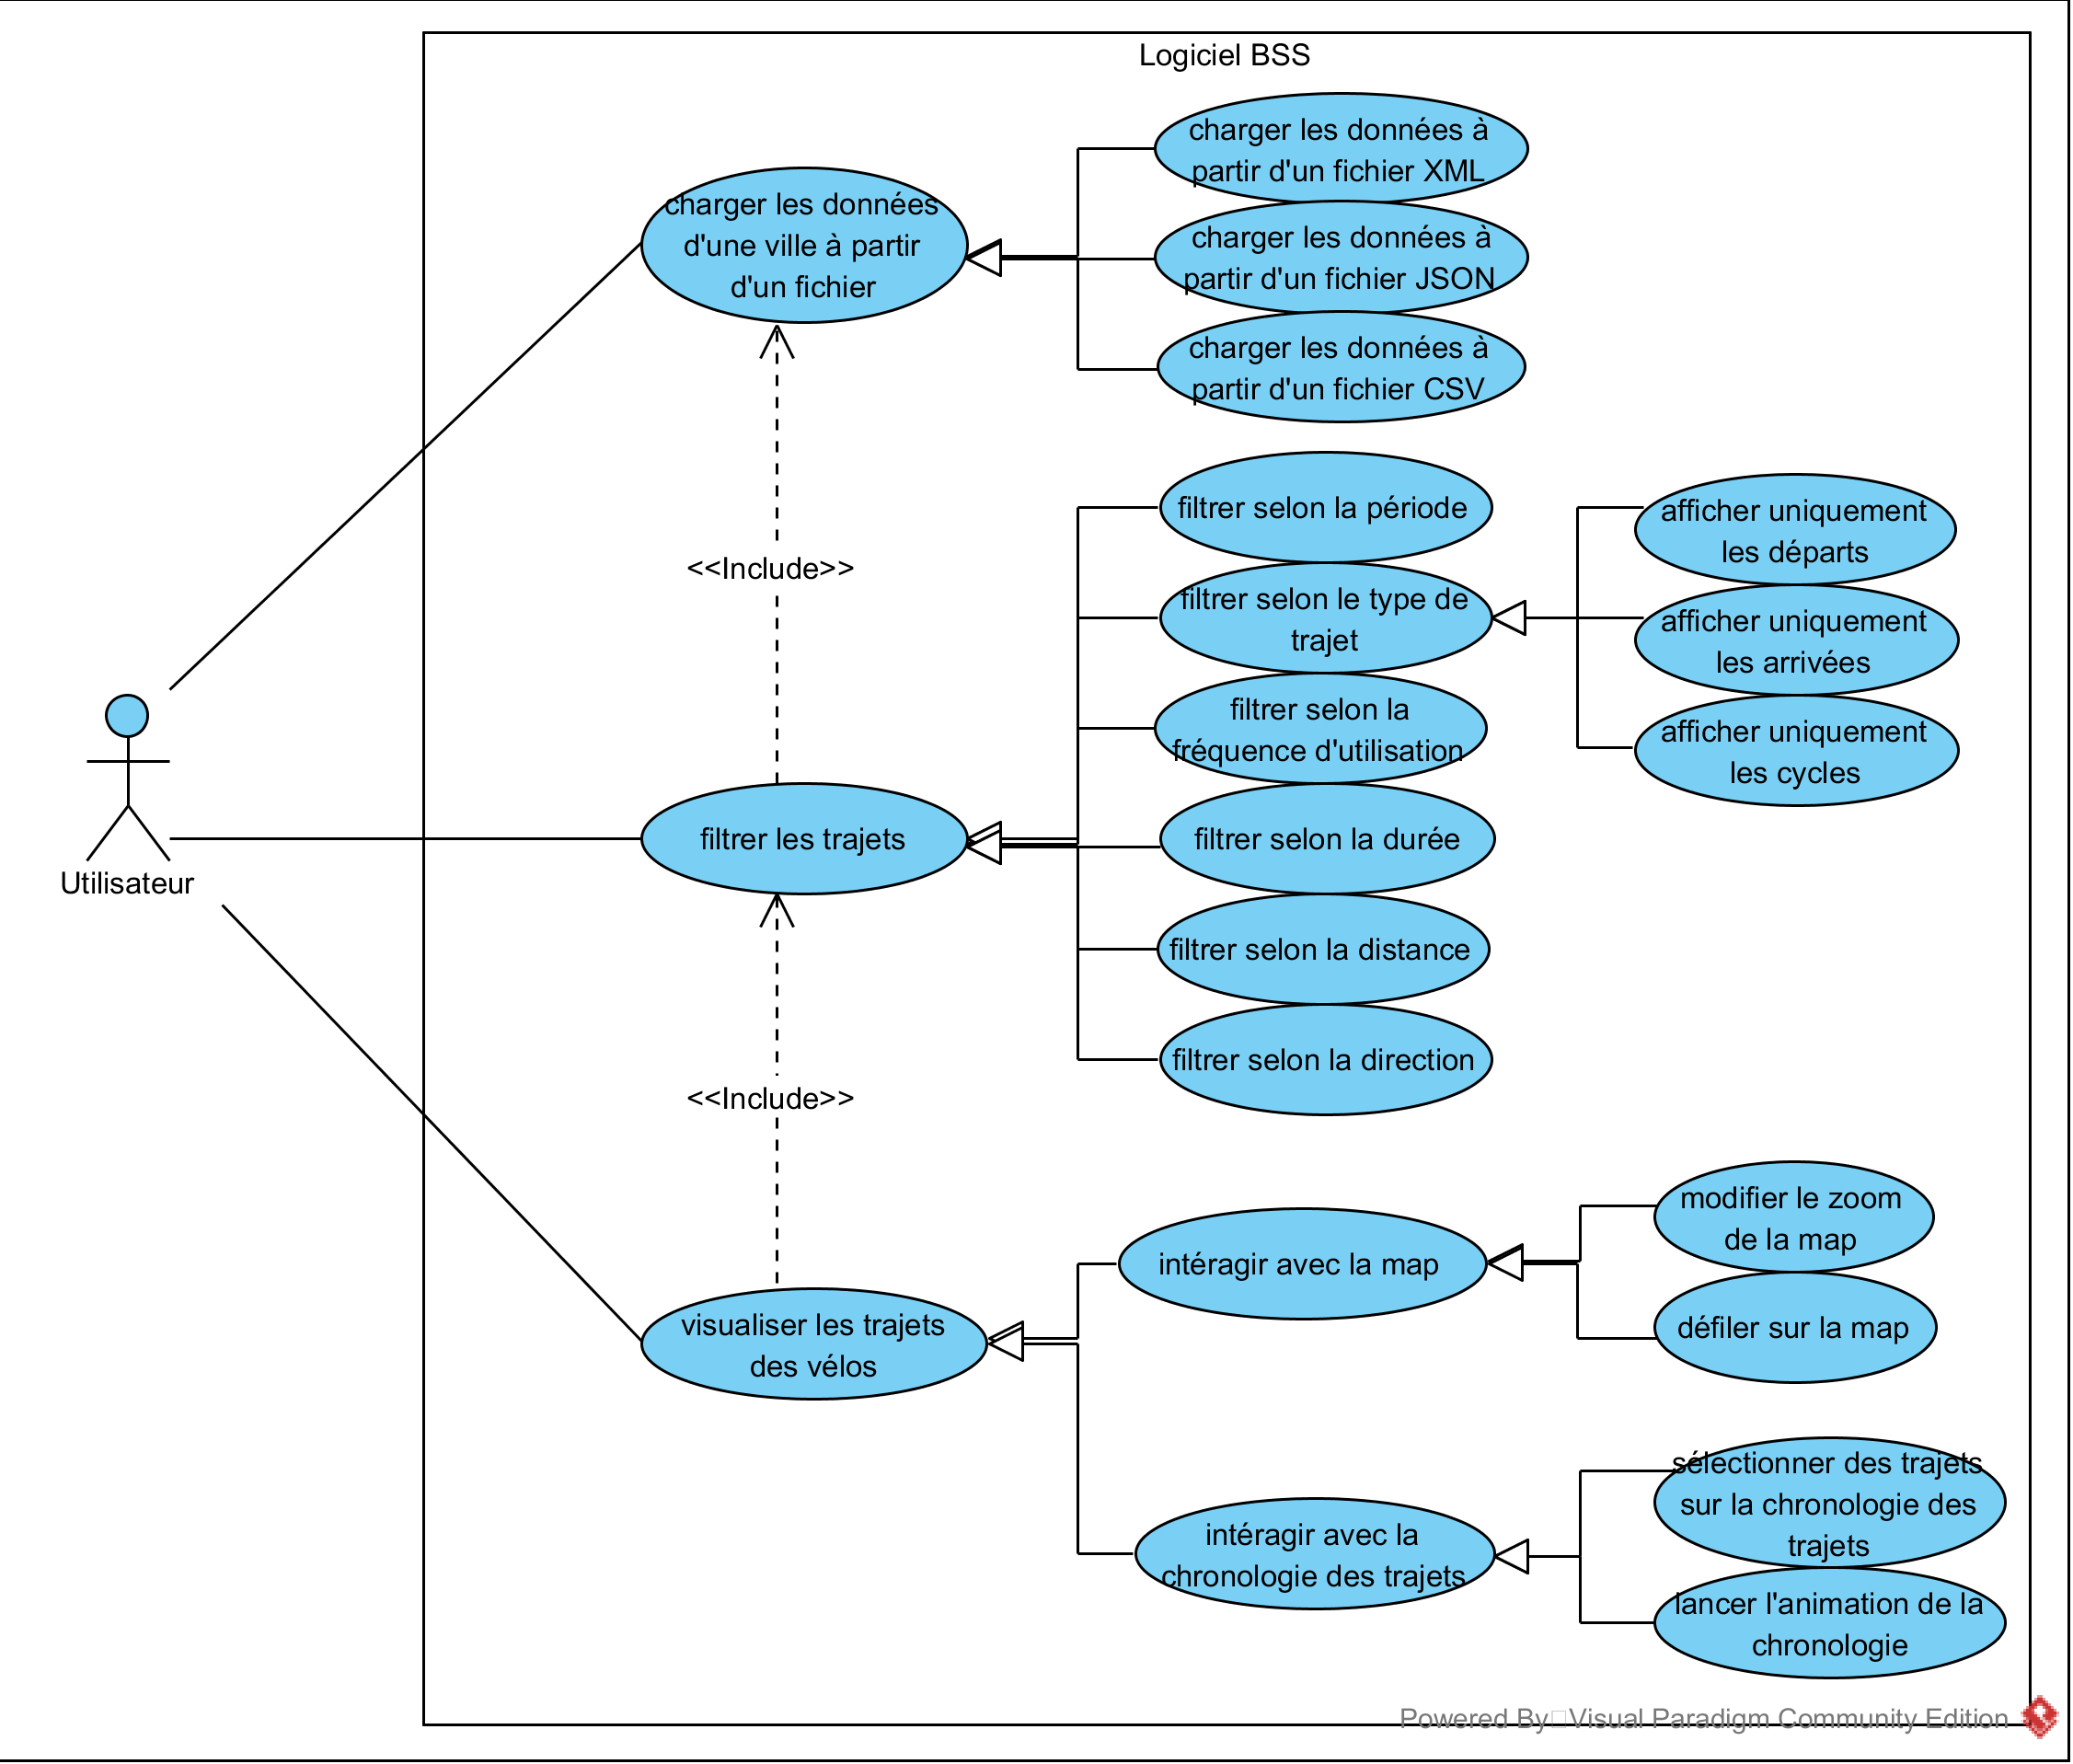
\includegraphics{use_case_1.png}
		\caption{Diagramme de cas d'utilisation.}
		\end{figure}

	\bibliography{bibliographie}

\end{document}
